  \documentclass[]{article}
\usepackage[makeroom]{cancel}
\usepackage{amsmath}
\usepackage[margin = 1.5 in]{geometry}
\usepackage{pgfplots}
\usepackage{tikz}
%opening
\title{Measuring the Fundamental Charge of An Electron}
\author{Andreas Badea, Mathew Harvey, Emilio Foley}

\begin{document}

\maketitle
\begin{center}
	\begin{tabular}{l r}
		Date Performed: & February 9, 2018 \\ % Date the experiment was performed
		Instructor: & Dr. Bradley Miller % Instructor/supervisor
	\end{tabular}
\end{center}

\section{Introduction}

In 1897, J.J. Thomson discovered the electron and measured its charge-to-mass ratio. But no one knew how to measure the charge of the electron. Thomson used clouds of charged water droplets and observed how fast they fell when gravity and an electric field were present. However, Thomson’s experiments produced only a very crude estimate of the electron’s charge. 

In 1906 Millikan, who was already a successful educator and textbook writer, was eager to make his mark also as a scientific researcher. Millikan saw the opportunity to make a significant contribution by improving upon Thomson’s results. Millikan believed that instead of measuring the charge on whole clouds of water like Thomson did, he could try to determine the charge on individual droplets. When he began his experiment, however, he noticed that water droplets evaporated too quickly for accurate measurement. 

\begin{figure}[ht]
	\begin{center}
		\includegraphics[width=3.5in]{diag}
	\end{center}
	\caption{Milikan's Experiment found the charge of very small drops of Oil}
\end{figure}

Fortunately, working with his graduate student Harvey Fletcher, Millikan figured out how to conduct his experiment with a substance that would evaporate more slowly: oil droplets produced by an atomizer. The oil droplets, injected into an air-filled chamber, fall or rise under the combined influence of gravity, viscosity of the air, and an electric field. The droplets pick up charge from the ionized air between the plates. By adjusting the electric field, Millikan could watch the droplets through a microscope and measure the time it takes for a droplet to fall or rise. After obtaining fall and rise time measurements, Millikan was able to calculate the charge on the droplet. 

Countless rounds of rigorous data collection later, Millikan reported the elementary charge to be 1.592 x 10-19 C, which is only slightly lower than the currently accepted value of 1.602 x 10-19 C. Millikan went on to win the 1923 Nobel Prize for his contribution to the field of electricity. The purpose of our experiment is to duplicate Millikan’s oil drop experiment, and hopefully verify his conclusion about the charge of the electron.
\section{Procedure}
ll materials were gathered before beginning experimentation. The materials included a high-voltage DC power source which can generate a minimum potential difference of 500V, a PASCO® Millikan Oil Drop Apparatus (Model AP-8210) which includes a low-viscosity mineral oil and an atomizer, a timer, and a stand to position the Apparatus at eye level. 

\begin{figure}[h]
	\begin{center}
		\includegraphics[width=3.1in]{pic}
	\end{center}
	\caption{ Setup for the PASCO® Millikan Oil Drop Apparatus
	}
\end{figure}


The Apparatus was placed on the stand and secured to prevent it from sliding as shown in the figure below. Afterwards, the DC power source was connected to an AC adapter connected to a wall socket and turned on to 0V. The power source was then connected to the Apparatus through the included plate charging switch, then the voltage on the Apparatus was slowly increased to 500V. Ambient light was then reduced by turning off the room lights and placing the device away from windows before turning on the halogen lamp which illuminates the droplet area. Oil was then poured into the atomizer and filled to approximately half of its maximum volume. To fill the droplet area with oil, the tip of the atomizer was placed over the hole in the covering of the droplet chamber and the bulb of the atomizer was given one full squeeze to release the oil. The oil was then seen either slowly rising or falling at a relatively constant velocity. The droplets were either put to rest by flipping the switch to its middle setting or allowed to change the direction of their velocities by flipping the switch to its opposite setting. 


Data was taken by recording the amount of time it took for one particular droplet to rise a chosen amount of distance on the order of one millimeter, then the time it took for the same droplet to fall the same distance. The data was assigned to the date it was taken, the ambient air pressure, the resistance of the thermistor, the separation of the electric plates, and the density of the oil as cited in the manual as well as its viscosity. Materials were put away after a total of eight rise and fall recordings.

\section{Data}
The time for small drops of ionized oil to fall and rise (under the influence of an electric field) were calculated these 

\begin{figure}[h]
	\centering
	\caption{Properties of Drops}
\begin{tabular}{ | c | c | c | c | c | c |}
	\hline 
	Drop \# & Date & Fall dist (mm) & Fall Time (s) & Rise dist (mm) & Rise Time (s) \\ \hline
	0 & 3-Feb-2013 & 0.50 & \( 33.0 \pm  0.8 \)  & 0.50 & \( 2.64 \pm 0.04 \) \\
	1 & 7-Feb-2018 & 1.00 & \( 18.9 \pm  0.5 \)  & 1.00 & \( 9.13 \pm 0.3 \) \\
	2 & 8-Feb-2018 & 0.50 & \(15 \pm  0.8 \)  & 0.50 & \( 3.35 \pm 0.15 \) \\
	3 & 8-Feb-2018 & 0.50 & \( 37.9 \pm  3.5 \)  & 1.00 & \( 4.85 \pm 0.03 \) \\
	4 & 8-Feb-2018 & 0.50 & \( 37.9 \pm  2.2 \)  & 0.50 & \( 6.19 \pm 0.17 \) \\
	5 & 8-Feb-2018 & 1.00 & \( 25.6 \pm  0.4 \)  & 1.00 & \( 6.44 \pm 0.11 \) \\
	6 & 3-Feb-2018 & 0.50 & \( 106 \pm 10 \)  & 0.50 & \( 2.31 \pm 0.6 \) \\
	7 & 8-Feb-2018 & 0.50 & \( 41.2 \pm  5.4 \)  & 0.50 & \( 4.72 \pm 0.19 \) \\ \hline	       
\end{tabular}
\caption{Properties of Days When Drops Were Collected}
\begin{tabular}{ | c | c | c | }
	\hline
	Date & Atmospheric Pressure (bar) & Thermistor Resistance (M\( \Omega\))\\ \hline
	3-Feb-2013 & 1017 & 2.04 \\
	7-Feb-2018 & 1018 & 1.98 \\
	8-Feb-2018 & 1030 & 1.95 \\ \hline
\end{tabular}
\end{figure}

These may be used to find the velocities of rise and fall which characterize the charge on each oil drop. It is also necessary to characterize the environmental conditions of the chamber in which the drops fall and rise. To do this, the pressure is measured, and the temperature inside the thermistor is estimated through a resistor inside. This may be also used to give an estimate of the viscosity of the air in the droplet chamber. Note that pressure may be adjusted slightly as the temperature within the thermistor is higher than the ambient temperature at which the pressure was measured, yielding a somewhat higher pressure within the thermistor. Generally this effect is relatively minimal and accounts for less that 0.5\% of the variance in the calculated charges

\begin{figure}
	
	\centering
	\caption{Other Relevant Information}
	\begin{tabular}{ | c | c | }
		\hline
		Voltage & \( 500 \pm 2\) V\\
		Viscosity of Air & \(1.844 \cdot 10^{-5} \mathrm{\frac{N \cdot s}{m^2}}\) \\
		Density of Oil & 866 \( \mathrm{\frac{kg}{m^3}}\)\\
		Gravitational Acceleration \footnotemark & 9.797 \( \mathrm{\frac{m}{s^2}}\) \\
		\hline
	\end{tabular}

\end{figure}




\section{Analysis}
\footnotetext{Density of Oil Viscosity of Air at measured temperature taken from model in AP-821A0 manual.
	\\
	Gravitational acceleration based on EMG2008 12th order model}
In order to determine the charge of the elemental charge particle, the charge on many small particles are computed and the distribution of the measured charges are compared. Of course, to do this one must first be able to find the charge on a single oil drop. This can be done simply using the velocities of the fall and the rise of the oil drop.

Both in free fall and when rising due to an electric charge the particles, being very small, reach a terminal velocity incredibly quickly. A terminal velocity is, of course, constant and thus the particle is experiencing no acceleration and has no net force acting upon it.

In free fall, the only forces acting upon the small drop of oil are the one due to gravity, \( m \, g \), and the one due to the coefficient of friction with the air. The relationship between the force of friction and the speed of free fall are assumed to be linearly related, with this frictional force, \(k \, v_f\) being proportional to the speed of freefall, \(v_f \), and some coefficient of friction with the air \( k \). These expressions give the equality,

\begin{equation}
m \, g = k \, v_f
\end{equation}

The rising oil drops are governed by a similar, if a bit more complicated, expression. These drops feel a third force, that of an electric field \( \mathbf{E} \). This force is simply \(\mathbf{E} \, q\), the product of the field and the charge of the particle \(q\) And, as rising instead of falling the direction of the force due to friction is downward rather than upward as before. This force due to friction is proportional to the speed of rising, \( v_r\). These give the equality

\begin{equation}
m \, g + k \, v_r = \mathbf{E} \, q.
\end{equation}

The coefficient of friction with the air is unknown and difficult to measure, it is thus necessary to remove it from the expression for charge. This may be accomplished by means of a simple substitution.

\begin{equation}
k = \frac{m \, g}{v_f} 
\end{equation}

Substituting this give a simple expression for the charge on an oil drop

\begin{equation}
q={\frac {m \, g \left( v_{f} + v_{r} \right) }{v_{f} \, E}}.
\end{equation}

This expression is simple, clean, and concise. But, it is also not particularly useful. It relies on the mass of the drops of oil, this is unknown, unmeasured, and by most conventional methods unmeasurable. This may seem problematic. But, If one assumes the oil drop to be a sphere of uniform density, then one may find the mass of the drop in terms of its radius, \(a\), and density, \(\rho\).

\begin{equation}
	m = \frac{4\pi}{3}\, \rho \, a^3.
\end{equation}
This may seem no more useful than the previous expression, if more convoluted. For the radius of the drops of oil is also not well known. However, there exists a relationship, Stoke’s Law, which attempts to model the falling speed of a droplet function of its radius that may be used. Stoke’s law claims that
\begin{equation}
a = \sqrt{\frac{9\, \eta \, v_f}{2 \, \rho \, g}},
\end{equation}
where \( \eta \) is the viscosity of the medium through which the drop falls. However, Stoke’s law is best applicable for droplets falling at a rate of greater than 0.1 cm/s, while the drops of oil that have been observed fall at a rate closer to \(10^{-5} \mathrm{m/s}\). This error may be fixed with a correction factor applied to the viscosity of air.
\begin{equation}
\eta_{eff} = \eta \, \left(  \frac{1}{1+\frac{b}{p \, a}} \right)
\end{equation}
Where \( p \) is the atmospheric pressure and b is a constant equal to \( 8.2 \times 10^{-3} \mathrm{Pa \cdot m} \). Substituting this into the expression for \(a\) yields the clunky and self referential formula :
\begin{equation}
a= \sqrt {{\frac {9 \, \eta\,v_{{f}}}{2 \, \rho\,g} \left( 1+{\frac {b}{p \, a}} \right) ^{-1}}}.
\end{equation}
With some rearrangements, this may be solved as a quadratic equation for \(a\). This is not too clean, but it yields an expression for \(a\).
\begin{equation}
a= \sqrt { \left( \frac{b}{2 \, p}  \right)^2 + \frac{9 \, \eta \, v_f }{2 \, \rho \, g} } - \frac{b}{2 \, p}
\end{equation}
This may be substituted into equation (5) to find the mass of the oil drop
\begin{equation}
m = \frac{4 \, \pi }{3} \, \rho \, \left( \sqrt { \left( \frac{b}{2 \, p}  \right)^2 + \frac{9 \, \eta \, v_f }{2 \, \rho \, g} } - \frac{b}{2 \, p} \right)^3
\end{equation}
And this into equation (4) along with the electric field for parallel plates \( \mathbf {E} = V / d\).
\begin{equation}
q = \frac{4 \, \pi }{3} \, \rho \, \left( \sqrt { \left( \frac{b}{2 \, p}  \right)^2 + \frac{9 \, \eta \, v_f }{2 \, \rho \, g} } - \frac{b}{2 \, p} \right)^3 {\frac { d \, g \left( v_{f} + v_{r} \right) }{v_{f} \, V}}
\end{equation}

\subsection{ \cancel{Erorrs} \xcancel{Erors} Errors}
It is necessarily and useful to quantify the error in the calculated charge. This may be estimated by estimating the error in each parameter and calculating the error contribution. This may be done my multiplying the error in each parameter by the partial derivative of the charge with respect to each parameter.
\subsubsection{Partial Derivatives}
\begin{equation}
\frac{\partial q}{\partial d } = \frac{q}{d}
\end{equation}
\begin{equation}
\frac{\partial q}{\partial V } = -\frac{q}{V}
\end{equation}
\begin{equation}
\frac{\partial q}{\partial p } = \frac{3 \, q \, b \sqrt{\rho \, g}}{ p \sqrt{b^2 \, \rho \, g +	18 \, \eta \, v_f \, p }}
\end{equation}
\begin{equation}
\frac{\partial q}{\partial v_r } = \frac{q}{v_r+v_f}
\end{equation}
\begin{equation}
\frac{\partial q}{\partial v_f } = q\, {\frac { \left( {b}^{2}g\rho\,v_{r}-27\,\eta\,{v_{f}}^{2}{p}^{2}-9
		\,\eta\,v_{{f}}{p}^{2}v_{{r}}-\sqrt {{b}^{2}\rho\,g+18\,\eta\,v_{{f}}{
				p}^{2}}\sqrt {\rho \, g}bv_{{r}} \right) \sqrt {\rho \, g}}{v_
		{{f}} \left( v_{{f}}+v_{{r}} \right)  \left( b\rho\,g-\sqrt {{b}^{2}
			\rho\,g+18\,\eta\,v_{{f}}{p}^{2}}\sqrt {\rho \, g} \right) \sqrt {
			{b}^{2}\rho\,g+18\,\eta\,v_{{f}}{p}^{2}}}}
\end{equation}
Each of these may be multiplied with the errors in their respective values and used to find their error contribution to the total calculated charge. If one is to assume independence in the parameters, one may choose to use the square root of the sum of the squares of these errors.
\subsection{Calculated Charges}
One may use the above sections to estimate the charge on each of the observed oil drops. Doing this yields the calculated charges

\begin{figure}[h]
	\centering
	\caption{Charges on drops of oil}
	\begin{tabular}{|c|c|}
		\hline
		Drop \# & Charge (C) \( \cdot 10^{-19}\) \\ \hline
		0 & \(3.01 \pm 0.07 \) \\
		1 & \(5.16 \pm 0.36 \) \\
		2 & \(4.42 \pm 0.26 \) \\
		3 & \(2.96 \pm 0.22 \) \\
		4 & \(1.25 \pm 0.07 \) \\
		5 & \(5.15 \pm 0.25 \) \\
		6 & \(1.43 \pm 0.53 \) \\
		7 & \(1.50 \pm 0.05 \) \\ \hline
		
	\end{tabular}
\end{figure}
This information is useful, but it is not immediately evident how to deduce the charge of a single electron simply from glancing at these numbers. It becomes beneficial to display these numbers in a means that best illustrates the integer multiples that one would expect to see in a world where charges come in discrete chunks. One may do this, simply by plotting the charges measured on each drop of oil from least to greatest such that near by charges may be compared to those with similar charges.
\begin{figure}[h]
	\centering
	\caption{Charges on Droplets of Oil}
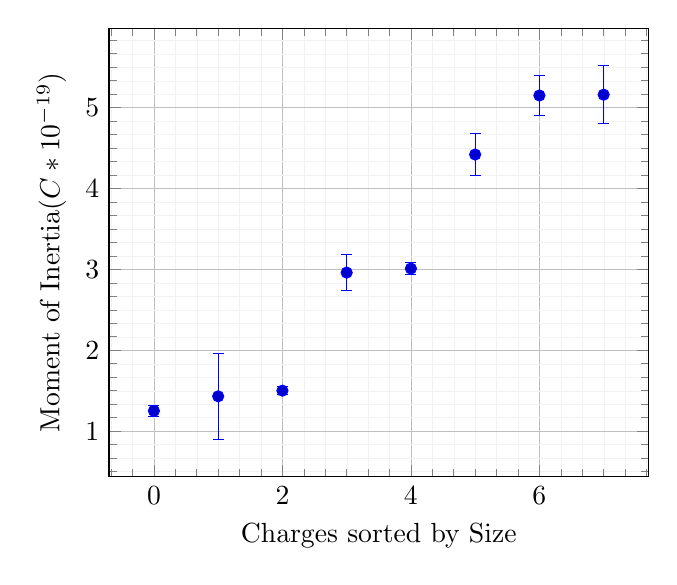
\begin{tikzpicture}
\begin{axis}[xlabel={Charges sorted by Size},
ylabel = {Moment of Inertia(\(C * 10^{-19}\))},
grid=both,
minor tick num=5,
grid style={line width=.1pt, draw=gray!10},
major grid style={line width=.2pt,draw=gray!50}]
\addplot+[only marks,
error bars/.cd,
x dir=both,x explicit,
y dir=both,y explicit,
]
table[x=x,y=y,,y error=yerror]
{
	x      y        yerror
	0    1.25 0.07
	1    1.43  0.53
	2    1.50  0.05
	3    2.96  0.22
	4    3.01 0.07
	5    4.42  .26
	6    5.15  0.25
	7    5.16   0.36
};
\end{axis}
\end{tikzpicture}

\end{figure}
\\
From this interpretation, one may rather quickly see that the charges are distributed on three strata. Droplets 4, 6 and 7 all appear to have roughly the same amount of charge on them, as do droplets 0 and 3. Droplets 1, 2. and 5 also appear to be in one grouping. One might also notice that the strata seem to be at charges roughly relating by integer multiples. Stratum 2 has roughly 2.1 times the charge as stratum 1, who has roughly a third (0.31) the charge of Stratum 3. This behavior suggests that the droplets of strata 1, 2 and 3 have 1, 2 and 3 fundamental charges on them respectively.

If one wishes to find the fundamental charge most accurately, one may choose to divide each measured droplet's charge by the estimated number of fundamental charges on that little droplet. Each drop should thus provide its own estimate for the electron's charge. And, A mean of this should provide a more accurate estimate for the fundamental charge on the electron and proton.
\begin{figure}
	\centering
	\caption{Estimation of Fundamental Charge Based on Each Electron}
\begin{tabular}{|c|c|}
	\hline
	Drop \# & Charge (C \(\cdot 10^{-19})\) \\ \hline
	0 &  \( 1.50 \pm 0.04\) \\
	1 &  \( 1.72 \pm 0.12\) \\
	2 &  \( 1.47 \pm 0.09\) \\
	3 &  \( 1.48 \pm 0.07\) \\
	4 &  \( 1.25 \pm 0.02\) \\
	5 &  \( 1.47 \pm 0.08\) \\
	6 &  \( 1.42 \pm 0.53\) \\
	7 &  \( 1.50 \pm 0.05\) \\
	\hline
\end{tabular}
\end{figure}

The mean of these values yields an average estimation of the fundamental charge of an electron to be \(1.48 \pm 0.12 \mathrm{\cdot 10^{-19} C}\).
\section{Conclusion}
This experiment estimated the fundamental charge of the electron to be \(1.48 \pm 0.12 \mathrm{\cdot 10^{-19} C}\). This is relatively close to its true value of \(1.60 \cdot 10^{-19} \mathrm{C}\) and the calculated value constitutes an error of 7.5\%. The true value of the charge of the electron is just within 1 standard deviation of the calculated charge for the drops. It is also worth noting the rather large amount of variance present in the charge estimate for each drop. This is partly because of the large amount of variance in the measured speeds. A At least qualitatively, the drops did not always appear to fall at a constant speed. Especially when falling, the drops appeared to rather randomly slow down, stop, or even drift upward for short periods of times. This might have to do with small disturbances and un-uniformities present in the distribution of the air. 

The effects of these are exacerbated because the oil drop is very small and thus more susceptible to these disturbances. This, somewhat random motion also, to a certain extent explains the underestimation in the charge on the drops. This stems from a overestimation of the fall speed and a underestimation of the time to fall. 

Consider a droplet which has a probability of falling down a little bit in every small period of time, and a smaller probability of staying still or going up in each small period of time. Naturally, this drop will trend downward, but will bob up and down anyway. It is very likely that this drop will pass through the same height quite a few times as it bobs up and down, but the impatient stop watch timer will chose to stop the drop as soon as the drop crosses the line, rather than the more difficult to estimate average line crossing time.

\begin{figure}[h]
	\centering
	\begin{center}
		\includegraphics[width=3.1in]{bia}
	\end{center}
	\caption{Randomly generated drop motion. Notice how the drop passes through the point -25 several times, the stopwatch would be stopped at the first and thus give a shorter time, higher speed, and smaller charge than if it had been stopped at the second.}
\end{figure}


Also, an impatient stop watch timer may chose to call time right before the drop has crossed the line rather than right after. This would also contribute to an underestimation of time. 

This, among other things, contributes to then underestimation of the charge on an electron.

\section{References}
“Millikan Oil Drop Apparatus - AP-8210A.” PASCO Scientific, 

\(\mathrm{www.pasco.com/prodCatalog/AP/AP-8210\_ millikan-oil-drop-apparatus}\)
\\ \\
Millikans Oil Drop Experiment. (n.d.). Retrieved February 10, 2018, from 

\(\mathrm{https://chemistry.tutorvista.com/inorganic-chemistry/millikan-s-oil-drop-experiment.html}\)
\\ \\
August, 1913: Robert Millikan Reports His Oil Drop Results. (n.d.). Retrieved February 9, 2018
\( \mathrm{https://www.aps.org/publications/apsnews/200608/history.cf  } \)
\\ \\
Oil drop experiment setup sketch | Socratic. (n.d.). Retrieved February 13, 2018, from 

\(\mathrm{https://socratic.org/questions/what-was-the-purpose-of-millikan-s-oil-drop-experiment}\)\\

\end{document}